\clearpage
\section{Close proximity detection}

The close proximity system consists of two main components, which are the readings from the ultrasonic sensors and the control of the rover using the motor controller.

%Picture of the three mounted ultra sonic sensors 

The three ultra sonic sensors are mounted as close as possible to each other, while still covering the greatest amount of vision on the front of the rover. Naturally, this causes two blind spot in between the ultrasonic sensors, to have an idea of how large the blind spot is, the following measurements and calculations have been made.

%Insert picture of calculations

\begin{figure}[H]
	\centering
	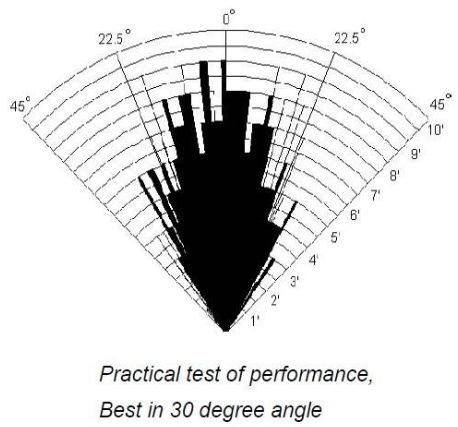
\includegraphics[width=.5\linewidth]{images/hcsr04angle.png}
\end{figure}
The ultrasonic sensor performs best at a $30\deg$ reading angle. This angle helps determine the area of which the ultrasonic sensor can read upon. The larger the angle, the less of a blindspot there will be when two or more ultrasonic sensors are placed on a line similar to how they are mounted on the rover\cite{hcsr40datesheet}.

\lstinputlisting[firstline=128, lastline=156, title=main, language=Python]{../code/autonomous-rover/obstacle-avoidance.py}

The core idea behind the current algorithm, is that per loop of the main code, the three ultrasonic sensors mounted on the front of the vehicle all gather three separate measurements. Then afterwards the measurements are compared in three different statements that will determine the direction. If the distance recorded by the left facing ultrasonic sensor is less than the threshold distance set as the variable \textit{avoid\_at}, the rover will then turn towards the right for the amount of seconds that the \textit{turn\_time} variable is set to. The same thing applies to the ultrasonic sensor faced to right, but instead the rover turns to the left when the threshold is exceeded.
If the threshold distance is exceeded at the center ultrasonic sensor, it determines whether the optimal path is to turn left or right depending on which direction has the largest distance measurement. This means that if an object is detected by the center ultrasonic sensor, the rover will then determine whether the distance measured to the left is greater than the distance measured to the right. The rover will then turn in the direction in which the distance measurement is greatest, since this theory means that the rover will have a longer distance until the rover meets an object.

%getdist()
\lstinputlisting[firstline=31, lastline=49, title=getdist(), language=Python]{../code/autonomous-rover/triple-ultrasonic-test.py}

At the start of the navigation loop seen in the \textit{main} code, the \textit{getdist()} function i run three separate times with different arguments, measurements are gathered every 200ms, where the datasheet recommends a measurements cycle of at least 60ms. The arguments are clearly labelled to help determine what measurement is coming from what ultrasonic sensor.
